\subsection{Six-line absorber}

\begin{figure}
\centering
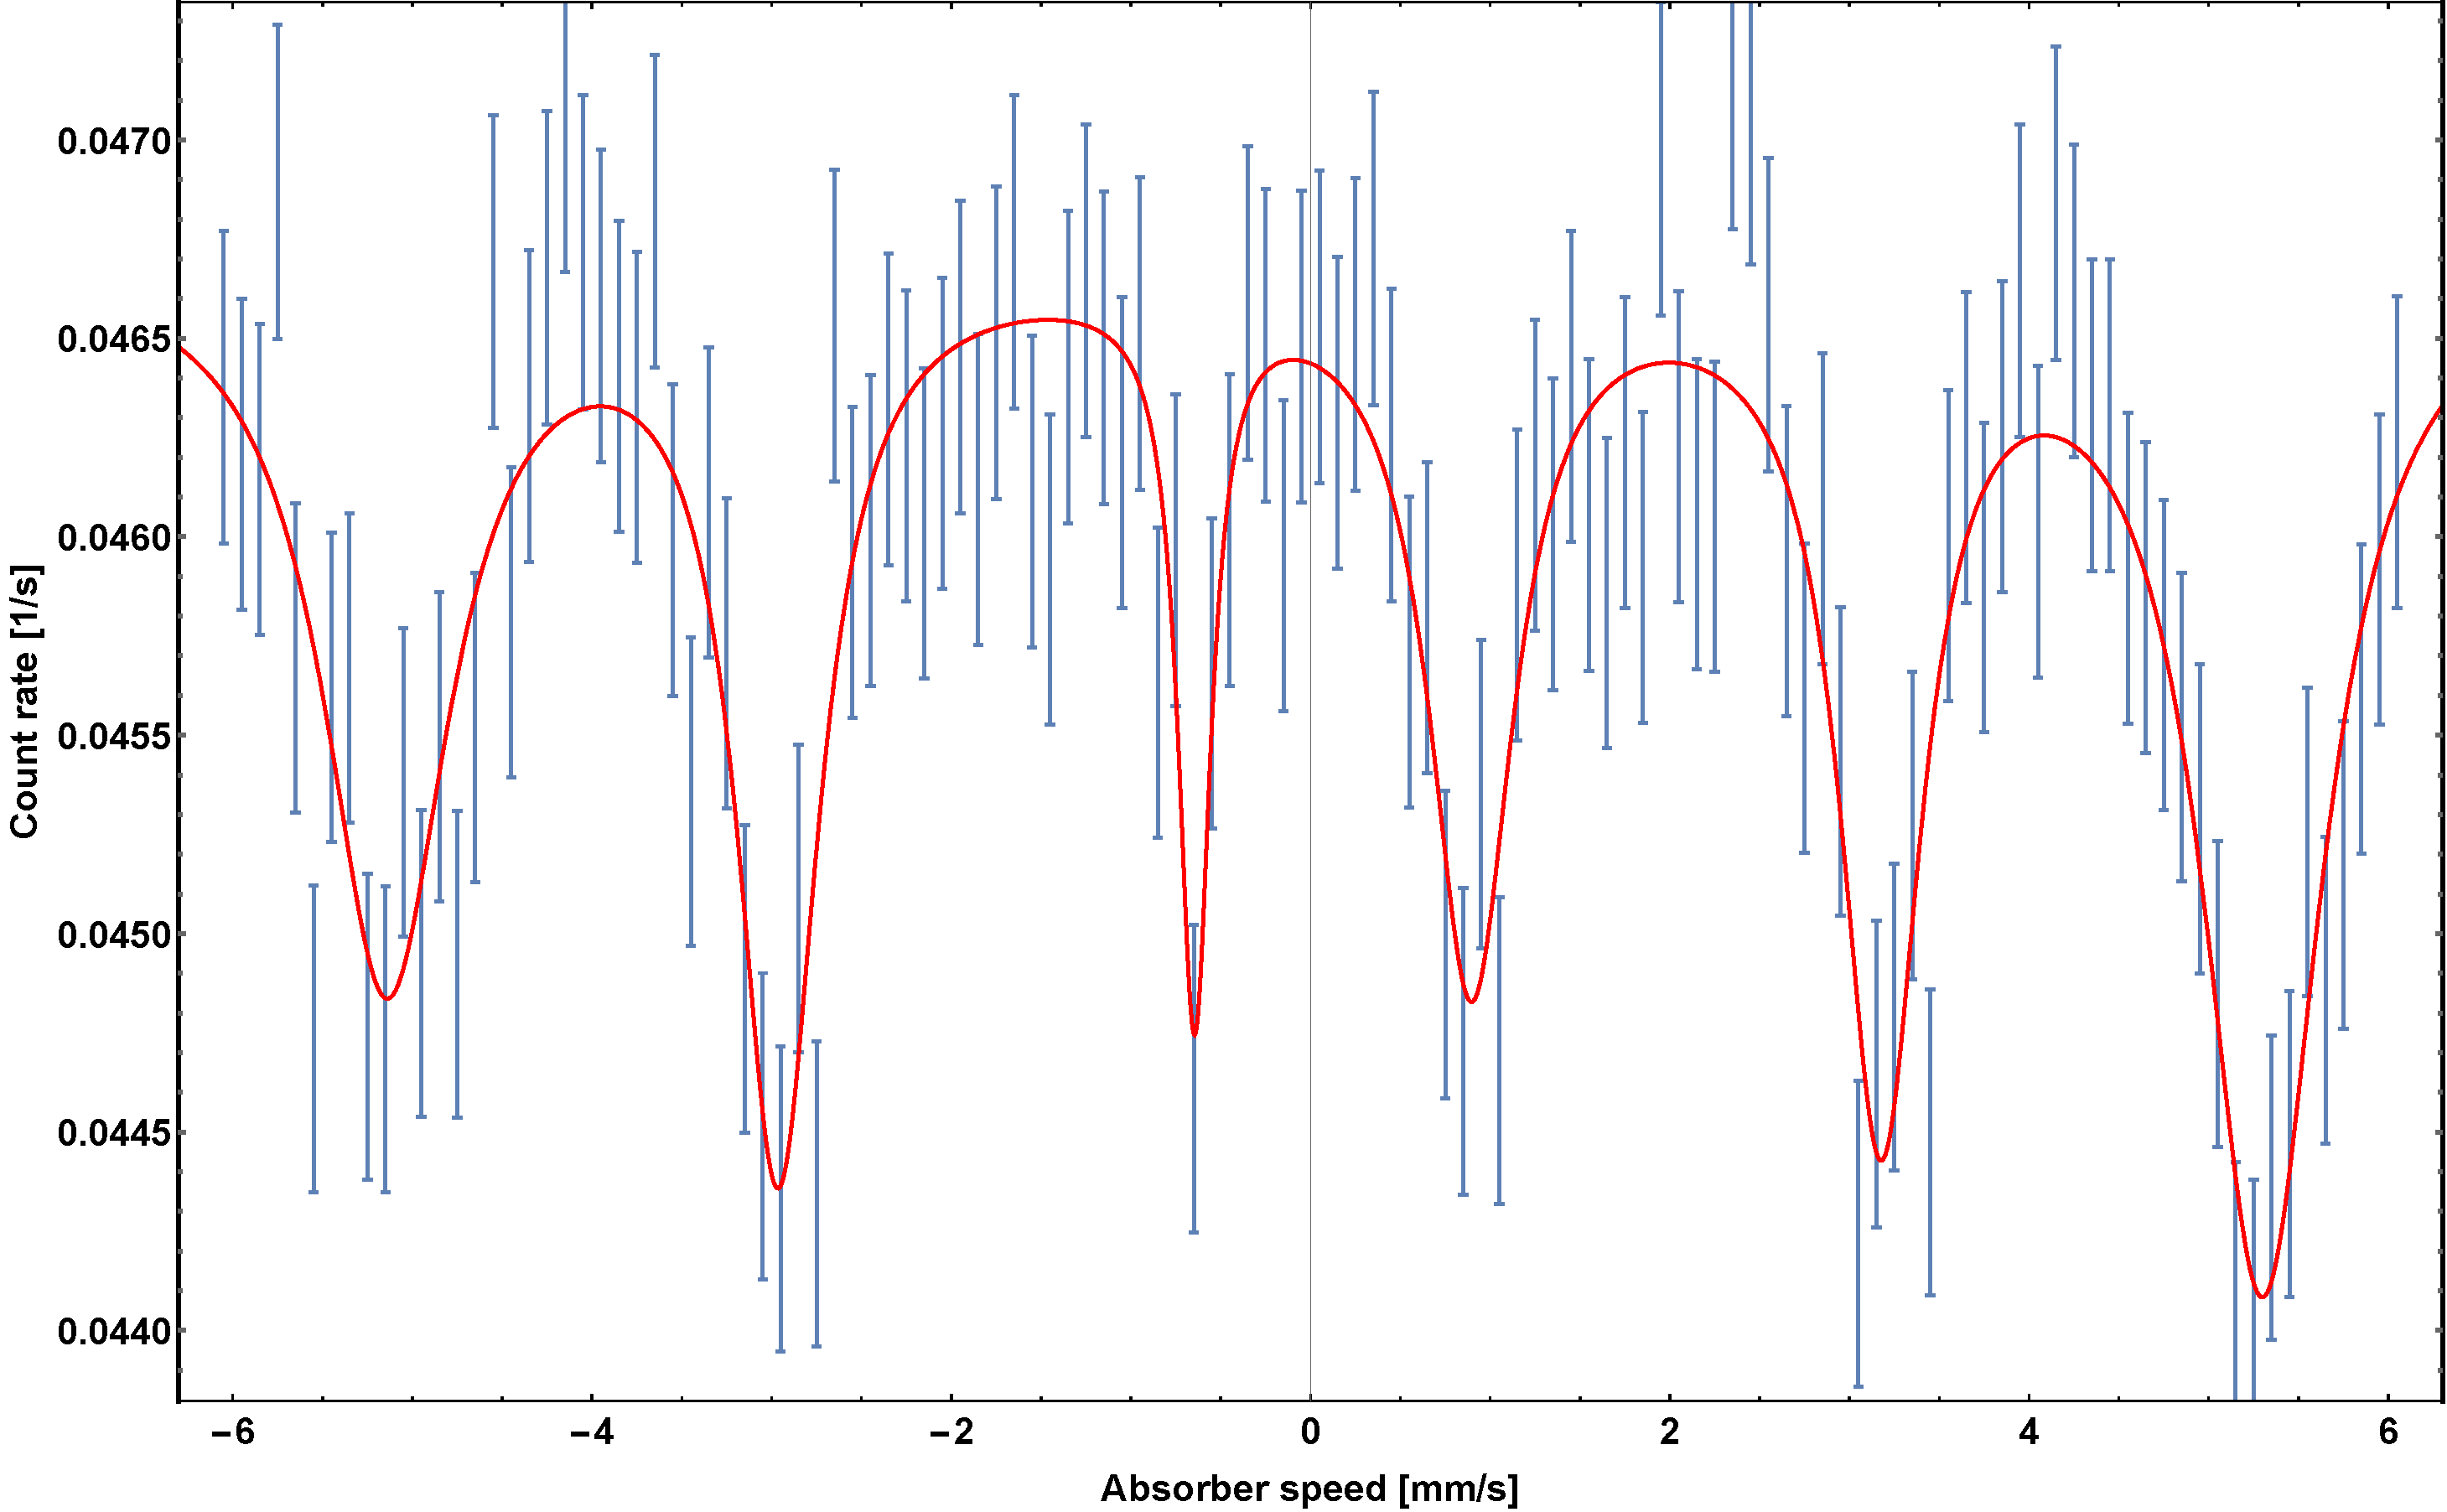
\includegraphics[width=1.0\linewidth]{graphics/natureisen}
\caption[Six-line absorber peaks]{The six-line absorber spectrum. A sum of 6 Lorentz functions was fitted to the data.}
\label{fig:natureisen}
\end{figure}
Figure \ref{fig:natureisen} shows the measurement results of the six-line absorber measurements. A sum of 6 Lorentz function, one for each peak, was fitted to the data. Gauss functions are to wide and due to the large uncertainties and the relatively low number of points per peak, the effort of doing Voigt fits is not warranted. The Lorentz fit describes the data well enough, with a $\chi^2$ value of 1.0. The peak positions and the corresponding energy shifts are listed in table \ref{tb:peakpositions}.\\
\begin{table}\centering
	\begin{tabular}{@{}lll@{}}
		\toprule
		Peak i & $v_i$ [mm/s]&$\Delta E$ [neV]\\
		\midrule
		1 & $-5.14\pm0.05$ & $-246.9\pm2.4$ \\
		2 & $-2.96\pm0.03$ & $-142.4\pm1.6$ \\
		3 & $-0.65\pm0.03$ & $-31.0\pm1.4$ \\
		4 & $0.90\pm0.04$ & $43.0\pm2.0$ \\
		5 & $3.18\pm0.03$ & $152.5\pm1.6$ \\
		6 & $5.30\pm0.03$ & $254.6\pm1.7$\\
		\bottomrule
	\end{tabular}
	\caption[Six-line absorber peak positions]{Positions of the peaks in the six-line absorber velocity spectrum.}
	\label{tb:peakpositions}
\end{table}
\subsubsection{Isomeric shift}
As the isomer shift is the offset from 0, three values can be determined here. One for the shift when comparing the first and sixth peak, on for the second and fifth and one for the third and forth. 
\begin{table}\centering
	\begin{tabular}{@{}lll@{}}
		\toprule
		Peaks & $v_{iso}$ [mm/s]&$E_{iso}$ [neV]\\
		\midrule
		6-1 & $0.08\pm0.03$ & $3.8\pm1.5$ \\
		5-2 & $0.106\pm0.023$ & $5.1\pm1.1$ \\
		4-3 & $0.125\pm0.025$ & $6.0\pm1.2$ \\
		\bottomrule
	\end{tabular}
	\caption[Six-line absorber: Isomer shift]{Isomer shifts of the six-line absorber.}
	\label{tb:isomershifts}
\end{table}
The weighted means of the values listed in table \ref{tb:isomershifts} are
\begin{align}
\overline{v}_{iso}&=\unit{(0.102\pm0.024)}{mm/s}\\
\overline{E}_{iso}&=\unit{(4.9\pm1.1)}{neV}
\end{align}
which both include their literature values $v_{iso}^{lit}=\unit{0.11}{mm/s}$ and $E_{iso}^{lit}=\unit{5.3}{neV}$ from the data sheet of the sample in their relatively large $1\sigma$ intervals.

\subsubsection{Magnetic moment}
Equation \ref{eq:HFS} yields
\begin{equation}
E_i=E_{iso}-E_{HFS}=E_{iso}-\left(\frac{\mu_em_e}{Ie}+\frac{\mu_gm_g}{I_g}\right)\cdot B
\end{equation}
which can be written using the velocities
\begin{equation}
v_i=v_{iso}-\frac{c}{E_0}\left(\frac{\mu_em_e}{Ie}+\frac{\mu_gm_g}{I_g}\right)
\end{equation}
The nuclear spins are$I_g=\nicefrac{1}{2}$ and $I_e=\nicefrac{3}{2}$. Table \ref{tb:peakqnumbers} shows the magnetic quantum numbers that correspond to the peaks.
\begin{table}\centering
	\begin{tabular}{@{}lll@{}}
		\toprule
		Peak & $m_e$&$m_g$\\
		\midrule
		1 & \nicefrac{3}{2} & \nicefrac{1}{2}\\
		2 & \nicefrac{1}{2} & \nicefrac{1}{2}\\
		3 & -\nicefrac{1}{2}& \nicefrac{1}{2}\\
		4 & \nicefrac{1}{2}& -\nicefrac{1}{2}\\
		5 & -\nicefrac{1}{2}& -\nicefrac{1}{2}\\
		6 & -\nicefrac{3}{2}& -\nicefrac{1}{2}\\
		\bottomrule
	\end{tabular}
	\caption[Quantum numbers of the peaks]{The magnetic quantum numbers corresponding to the peaks.}
	\label{tb:peakqnumbers}
\end{table}
The formulas still contain the unknown magnetic field. One can now calculate the velocity differences of the corresponding peaks
\begin{align}
\Delta v_a=v_6-v_1=\frac{2c}{E_0}&\left(\mu_g-\mu_e\right)B\\
\Delta v_b=v_5-v_2=\frac{2c}{E_0}&\left(\mu_g-\frac{\mu_e}{3}\right)B\\
\Delta v_c=v_4-v_3=\frac{2c}{E_0}&\left(\mu_g+\frac{\mu_e}{3}\right)B
\label{eq:thevaformulas}
\end{align}
With these three variables, there are three possible combinations to get formulas for the magnetic moment of the excited state. 
\begin{align}
\frac{\Delta v_a}{\Delta v_b}&=\frac{\mu_g-\mu_e}{\mu_g-\frac{\mu_e}{3}}\\
\frac{\Delta v_b}{\Delta v_c}&=\frac{\mu_g-\mu_e}{\mu_g+\frac{\mu_e}{3}}\\
\frac{\Delta v_c}{\Delta v_a}&=\frac{\mu_g+\frac{\mu_e}{3}}{\mu_g-\frac{\mu_e}{3}}
\end{align}
The magnetic moment of the ground state is given in \cite{stone} as $\mu_g=(0.09044\pm0.0007)\cdot\mu_N$, where the nuclear magneton is $\mu_N=\unit{3.152\cdot10^{-8}}{eV/T}$. Solving these separate formulas for the magnetic moment of the excited state and applying standard Gaussian error propagation yields (in units of $\mu_N$)
\begin{align}
\frac{\Delta v_a}{\Delta v_b}\Rightarrow \mu_e&=\mu_g\frac{3\Delta v_a-\Delta v_b}{\Delta v_a-3\Delta v_b}=\unit{(0.146\pm0.005)}{\mu_N}\\
\frac{\Delta v_b}{\Delta v_c}\Rightarrow\mu_e&=3\mu_g\frac{\Delta v_c-\Delta v_b}{\Delta v_c+\Delta v_b}=\unit{(0.162\pm0.003)}{\mu_N}\\
\frac{\Delta v_c}{\Delta v_a}\Rightarrow\mu_e&=\mu_g\frac{\Delta v_c-\Delta v_a}{\Delta v_a/3+\Delta v_c}=\unit{(0.160\pm0.003)}{\mu_N}
\end{align}
Stone \cite{stone} lists the magnetic moment of the excited state as $\mu_e=\unit{(-0.1549\pm0.0002)}{\mu_N}$.
All values enclose this value at least in their $3\sigma$ intervals. 

\subsubsection{The magnetic field at the nucleus}
With the magnetic moments known, the magnetic fields can now be calculated from the formulas in equation \ref{eq:thevaformulas}
\begin{align}
	B_a&=\unit{(33.7\pm0.7)}{T}\\
	B_b&=\unit{(32.4\pm0.4)}{T}\\
	B_c&=\unit{(31.7\pm1.5)}{T}
\end{align}
which are all within $2\sigma$ of the literature value $B_{lit}=\unit{33}{T}$\cite{Fultz}.
